\documentclass[prl,twocolumn]{revtex4-1}

\usepackage{graphicx}
\usepackage{color}
\usepackage{latexsym,amsmath}

\definecolor{linkcolor}{rgb}{0,0,0.65} %hyperlink
\usepackage[pdftex,colorlinks=true, pdfstartview=FitV, linkcolor= linkcolor, citecolor= linkcolor, urlcolor= linkcolor, hyperindex=true,hyperfigures=true]{hyperref} %hyperlink%

\makeatletter
\renewcommand{\section}{\@startsection{section}{1}{\z@}%
	{-3.5ex \@plus -1ex \@minus -.2ex}{2.3ex \@plus.2ex}%
	{\normalfont\bfseries\raggedright}}

% Ripristina la definizione di \subsection per allineamento a sinistra
\renewcommand{\subsection}[1]{%
	\@startsection{subsection}{2}{\z@}%
	{3.5ex \@plus 1ex \@minus .2ex}{-1em}%
	{\normalfont\bfseries\raggedright #1}%
}

\makeatother


\begin{document}

\title{GROUP2505 -- Log-likelihood analysis for Restricted Boltzmann Machines}



\author{Elias Maria Bonasera}
\author{Alberto Casellato}
\author{Nicola Garbin}
\author{Francesco Pazzocco}

\date{\today}


\begin{abstract}
  Here, in the ``abstract'' (more or less of 8 lines), there should be a short summary of the work and of its main findings. In a paper, the abstract is important also for attracting potential readers, hence it is convenient to start it with some catchy statement. ---
 The rest of this text has the double purpose of (a) providing a template for the assignment latex, and (b) introducing how to structure the backbone of the text and explaining some details of this assignment. The ``zzz'' fill the space to show a typical (but not rigid) extension of the parts.
  zzzzzzzzzzzzzzz zzzzz zzzzzzzzzz zzzzzzz z zzzzzzzzzzz zzzz zzzzzzzzz
  zzzzzzzzzzzzzzz zzzzz zzzzzzzzzz zzzzzzz z zzzzzzzzzzz zzzz zzzzzzzzz
  zzzzzzzzzzzzzzz zzzzz zzzzzzzzzz zzzzzzz z zzzzzzzzzzz zzzz zzzzzzzzz
  zzzzzzzzzzzzzzz zzzzz zzzzzzzzzz zzzzzzz z zzzzzzzzzzz zzzz zzzzzzzzz.
\end{abstract}

\maketitle

\section{1. Introduction}
The main goal of this assignment is to explore how the performance of an RBM changes for different choices of the hyperparameters of the model, using the MNIST digits as the database; in particular, using the log-likelihood evaluation, we explore the trend of the model during the learning process as the number of epochs increases.

In section \emph{2.} it is exposed a brief insight of the Restricted Boltzmann Machines architecture. The log-likelihood is introduced in this section as it is adopted both to estimate the performance of the model and as an evaluation of $\nabla_{\boldsymbol{\theta}}{E(\boldsymbol{\theta})}$ in optimizers (see Eq.~\ref{eq:sgd} and Eq.~\ref{eq:rmsprop}). Subsection \emph{3.1.} is opened with the explicit expression for the partition function $Z$ in the Bernoulli case (Eq.~\ref{eq:Z_function_bernulli}) and then it regards theoretical insight about setting parameters of the model. In subsection \emph{3.2.} operative choices regarding simulations are discussed, including numerical methods adopted to prevent computation errors. The explicit expression for the partition function $Z$ in the Spin case (Eq.~\ref{eq:Z_function_spin}) is introduced in this subsection, since it is approximated in a similar way compared to the Bernoulli case. In section \emph{4.} results concerning the log-likelihood are discussed, dependent on number $L$ of hidden units (Figure~\ref{fig:L_of_L}), CD steps number (Figure~\ref{fig:final_L_of_CD}), $\gamma$ parameter (..), learning rate (..), optimizers choice (..), Bernoulli vs Spin case (..), POTTS on/off for SGD optimizer (..) and POTTS on/off for RMSprop optimizer (..).


\section{2. Restricted Boltzmann Machines} \label{RBM}
%\noindent\textbf{1.2 Restricted Boltzmann Machines}

\setcounter{equation}{0}

Restricted Boltzmann Machines (RBM) are a powerful kind of generative models designed to accomplish training processes relatively fast. In RBMs, a set of $D$ binary visible units $i$ of state $\{v_i\}_{i=1, ..., D}$ is symmetrically connected to a set of $L$ binary hidden units $\mu$ of state $\{h_\mu\}_{\mu=1, ..., L}$; the continuos weight $w_{i\mu}$ quantifies the strength between unit $i$ and unit $\mu$ (see Figure~\ref{fig:RBM_architecture}). RBMs use an energy function to define the probability distribution over the input data \cite{pap1} \cite{pap2}.

%%%%%%%%%%%%%%%%%%%
\begin{figure}[!tb]
	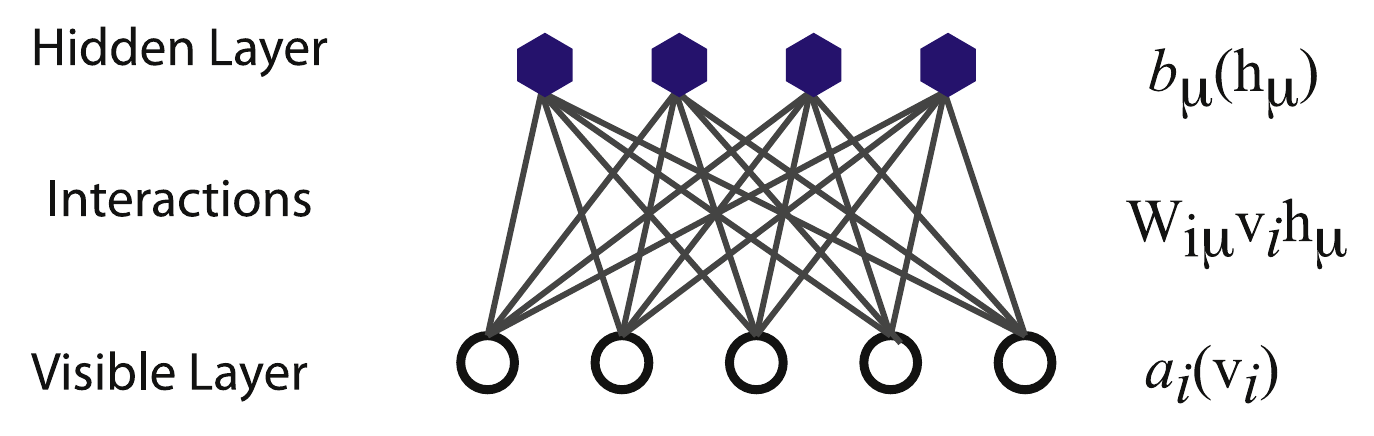
\includegraphics[width=0.465\textwidth]{RBM_structure.png}
	\caption{A Restricted Boltzmann Machine (RBM) is made up of visible units, denoted as $v_i$, and hidden units, represented as $h_\mu$. These units engage with one another through interactions characterized by the weights $w_{i\mu}$. Notably, there are no direct interactions among the visible units or among the hidden units themselves.}
	\label{fig:RBM_architecture}
\end{figure}
%%%%%%%%%%%%%%%%%%%

In the training process the energy of the configuration is minimized by adjusting the parameters $\boldsymbol{\theta}$. One of the most adopted training algorithm is Contrastive Divergence which allows to approximate the gradient of the likelihood to update the parameters. During this process, a cyclic Gibbs sampling is performed setting the visible units given the hidden ones and vice versa, according to the following probabilities $p$:

\begin{equation}
	p(h_\mu=1\ |\ \mathbf{v}) = \sigma(b_\mu + \sum_{i}v_iw_{i\mu})
	\label{eq:p_of_h}
\end{equation}
\begin{equation}
	p(v_i=1\ |\ \mathbf{h}) = \sigma(a_i + \sum_{\mu}h_{\mu}w_{i\mu})
	\label{eq:p_of_v}
\end{equation}

where $\sigma(x)=1/(1+e^{-x})$ is the logistic sigmoid function, $a_i$ is the bias of the $i$-th visible unit and $b_\mu$ is the bias of the $\mu$-th hidden unit; they act shifting the sigmoid function $\sigma(x)$. The absence of links among units of the same type simplifies the training process. Moreover, the number of iterations of Eq.~\ref{eq:p_of_h} and Eq.~\ref{eq:p_of_v} can be setted to $2$ if real data is used to fix $\{v_i\}_{i=1, ..., D}$ in the first place.

The goodness of a model is evaluated by computing the log-likelihood $\mathcal{L}$ of the data:

\begin{equation}
	\mathcal{L}=\frac{1}{M}\sum_{m=1}^{M}{\ell_{\theta}(v^{(m)})}
	\label{eq:Loglikelihood}
\end{equation}
\begin{equation}
	\ell_{\theta}(v^{(m)})=\log\sum_{h}{e^{-E(v,h)}-\log{Z}}
	\label{eq:loglikelihood}
\end{equation}

where $M$ is the number of data points, $Z$ is the partition function, $E(v,h)$ in the exponential argument $e^{-E(v,h)}=G(h)\prod_{i}{e^{H_i(h)v_i}}$ is the energy function, with $G(h)=\prod_{\mu}{e^{b_{\mu}h_{\mu}}}$ and $H_i(h)=a_i+\sum_{\mu}w_{i\mu}h_\mu$, and, in Eq.~\ref{eq:loglikelihood}, the index $h$ of the summation represents each possible state of the hidden layer.

%%%%%%%%%%%%%%%%%%%
\begin{figure}[!tb]
	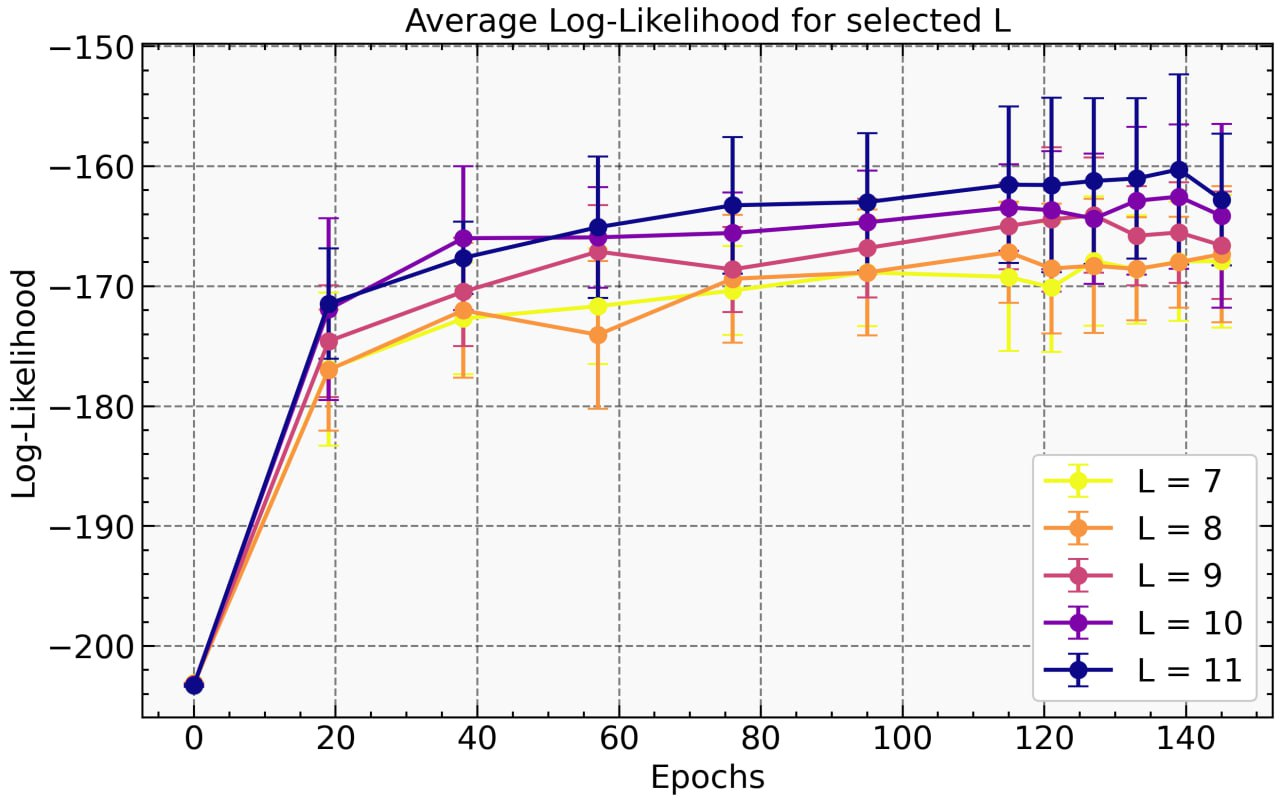
\includegraphics[width=0.44\textwidth]{L_of_epochs.jpg}
	\caption{The evolution of the log-likelihood over training epochs for each L is shown. The curves represent the average log-likelihood across 10 stochastically distinct runs.}
	\label{fig:L_of_epochs}
\end{figure}
%%%%%%%%%%%%%%%%%%%

%%%%%%%%%%%%%%%%%%%
\begin{figure}[!tb]
	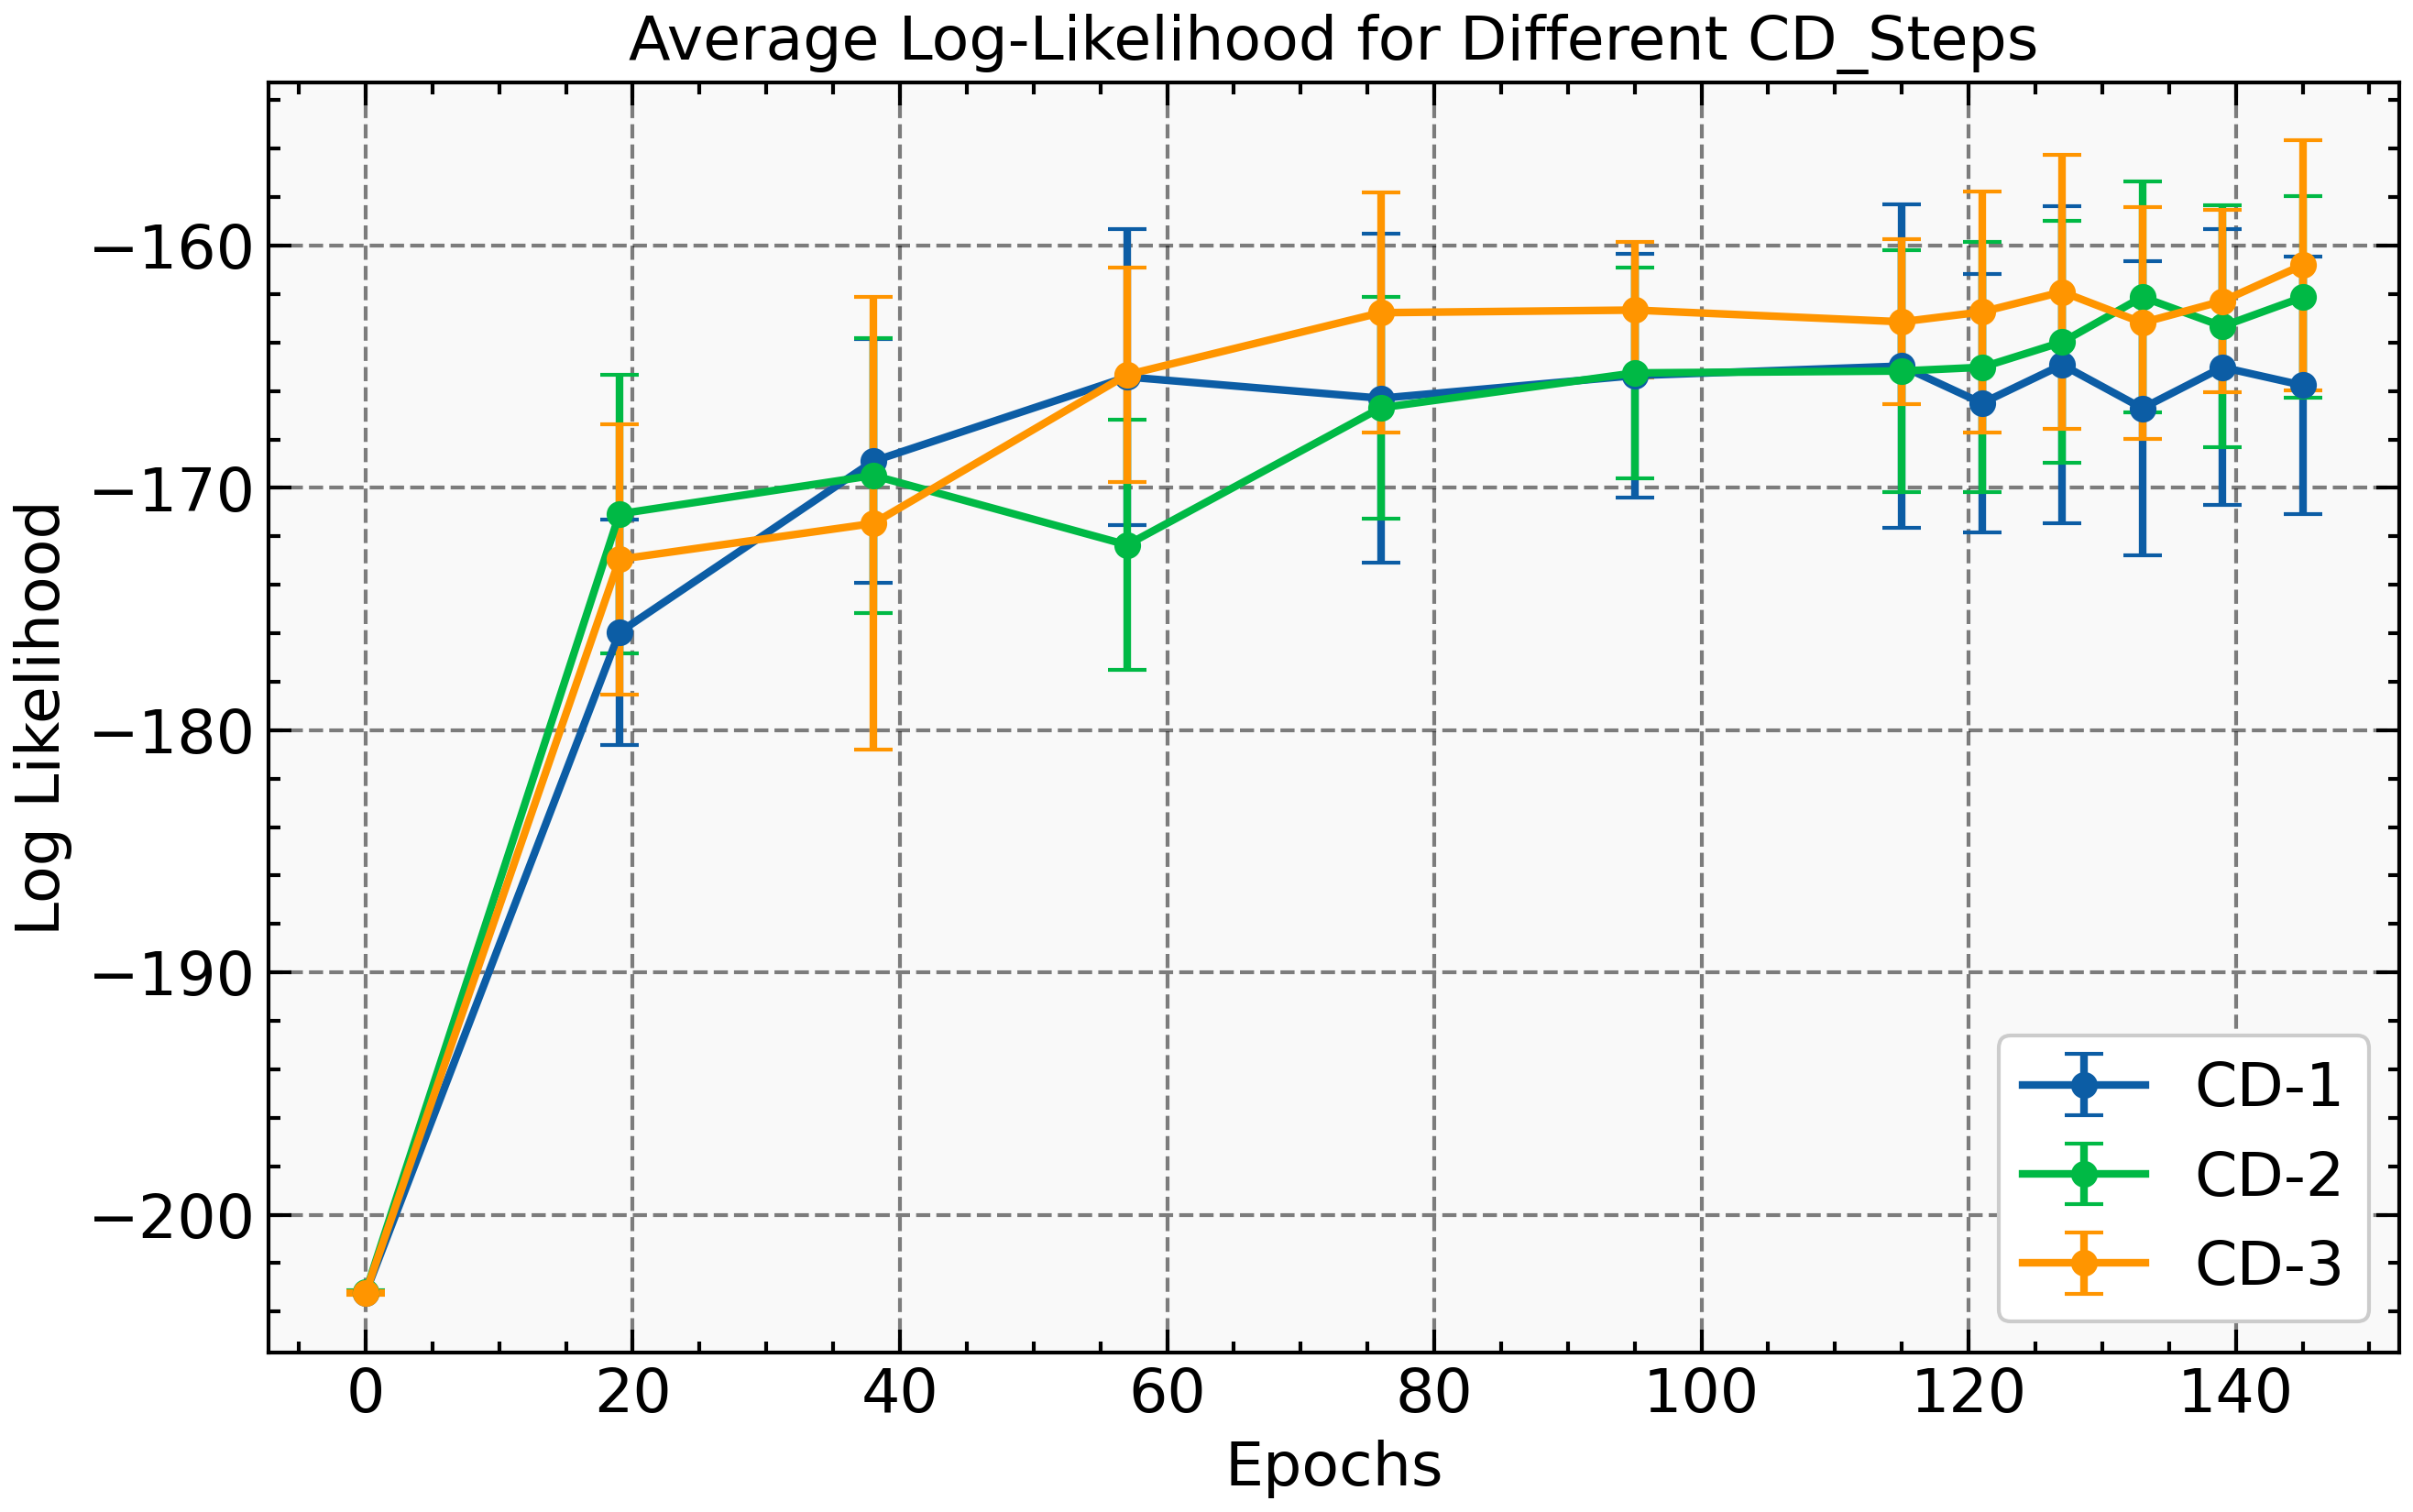
\includegraphics[width=0.44\textwidth]{L_of_CD.png}
	\caption{The figure shows the evolution of the log-likelihood over training epochs for different numbers of CD steps. The curves represent the average log-likelihood across 10 stochastically distinct runs.}
	\label{fig:L_of_CD}
\end{figure}
%%%%%%%%%%%%%%%%%%%

\section{3. Methods}
\noindent\textbf{3.1. Theoretical implementation}
\\
\\
Regarding the computation of the partition function $Z$ (in Eq.~\ref{eq:loglikelihood}), its implementation depends on the set of values which each unit can be set on. Since the direct computation of the $Z$ function is unfeasible, due to the summation of all possible state combinations of the system, a possible approach is to split the summation separately over states $v$ and $h$.

For the Bernulli case the units can assume the values $\{0,1\}$ and the partition function form can be manipulated to obtain the following expression:

\begin{equation}
	Z=\sum_v\sum_h{e^{-E(v,h)}}=q^D\sum_h{G(h)\prod_{i=1}^D{\frac{1+e^{H_i(h)}}{q}}}
	\label{eq:Z_function_bernulli}
\end{equation}

%%%%%%%%%%%%%%%%%%%
\begin{figure}[!tb]
	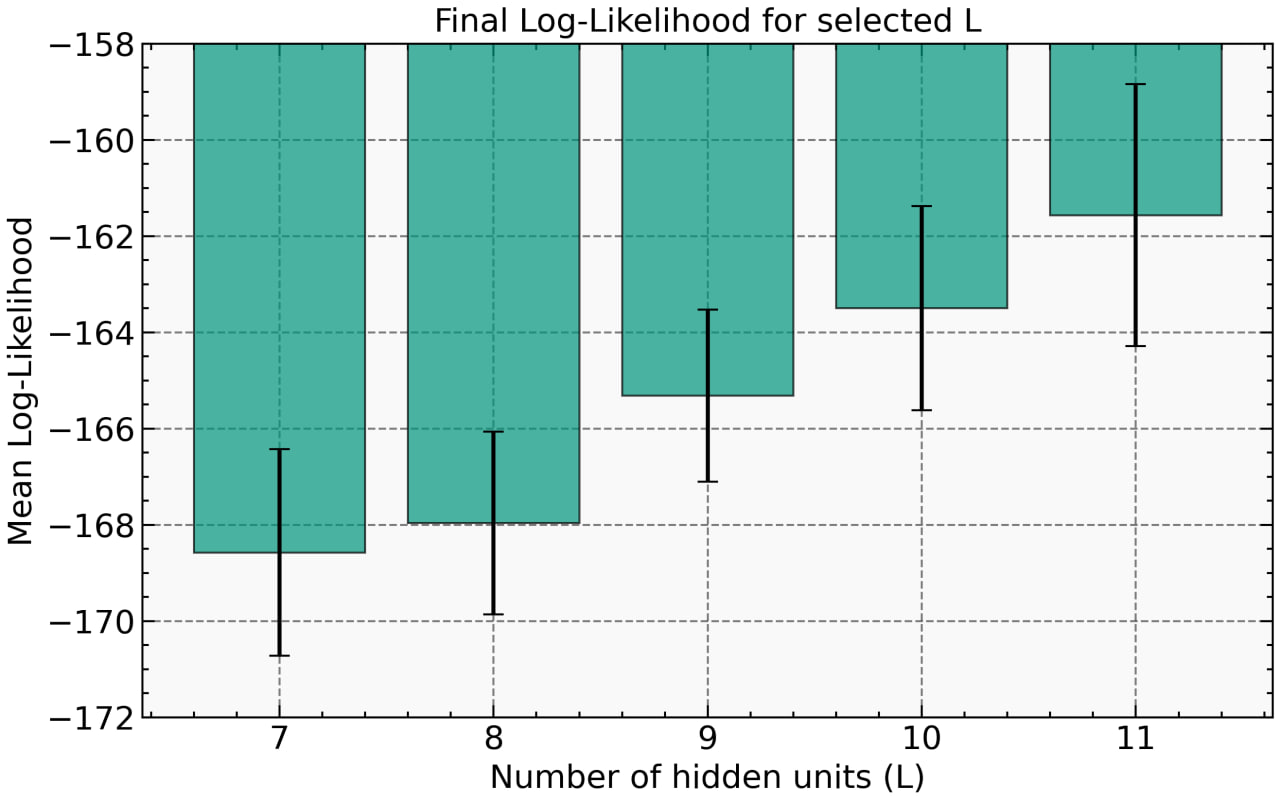
\includegraphics[width=0.44\textwidth]{L_of_L.jpg}
	\caption{Bar chart displaying the weighted mean and standard deviation of the log-likelihood over the last epochs for different values of L.}
	\label{fig:L_of_L}
\end{figure}
%%%%%%%%%%%%%%%%%%%

%%%%%%%%%%%%%%%%%%%
\begin{figure}[!tb]
	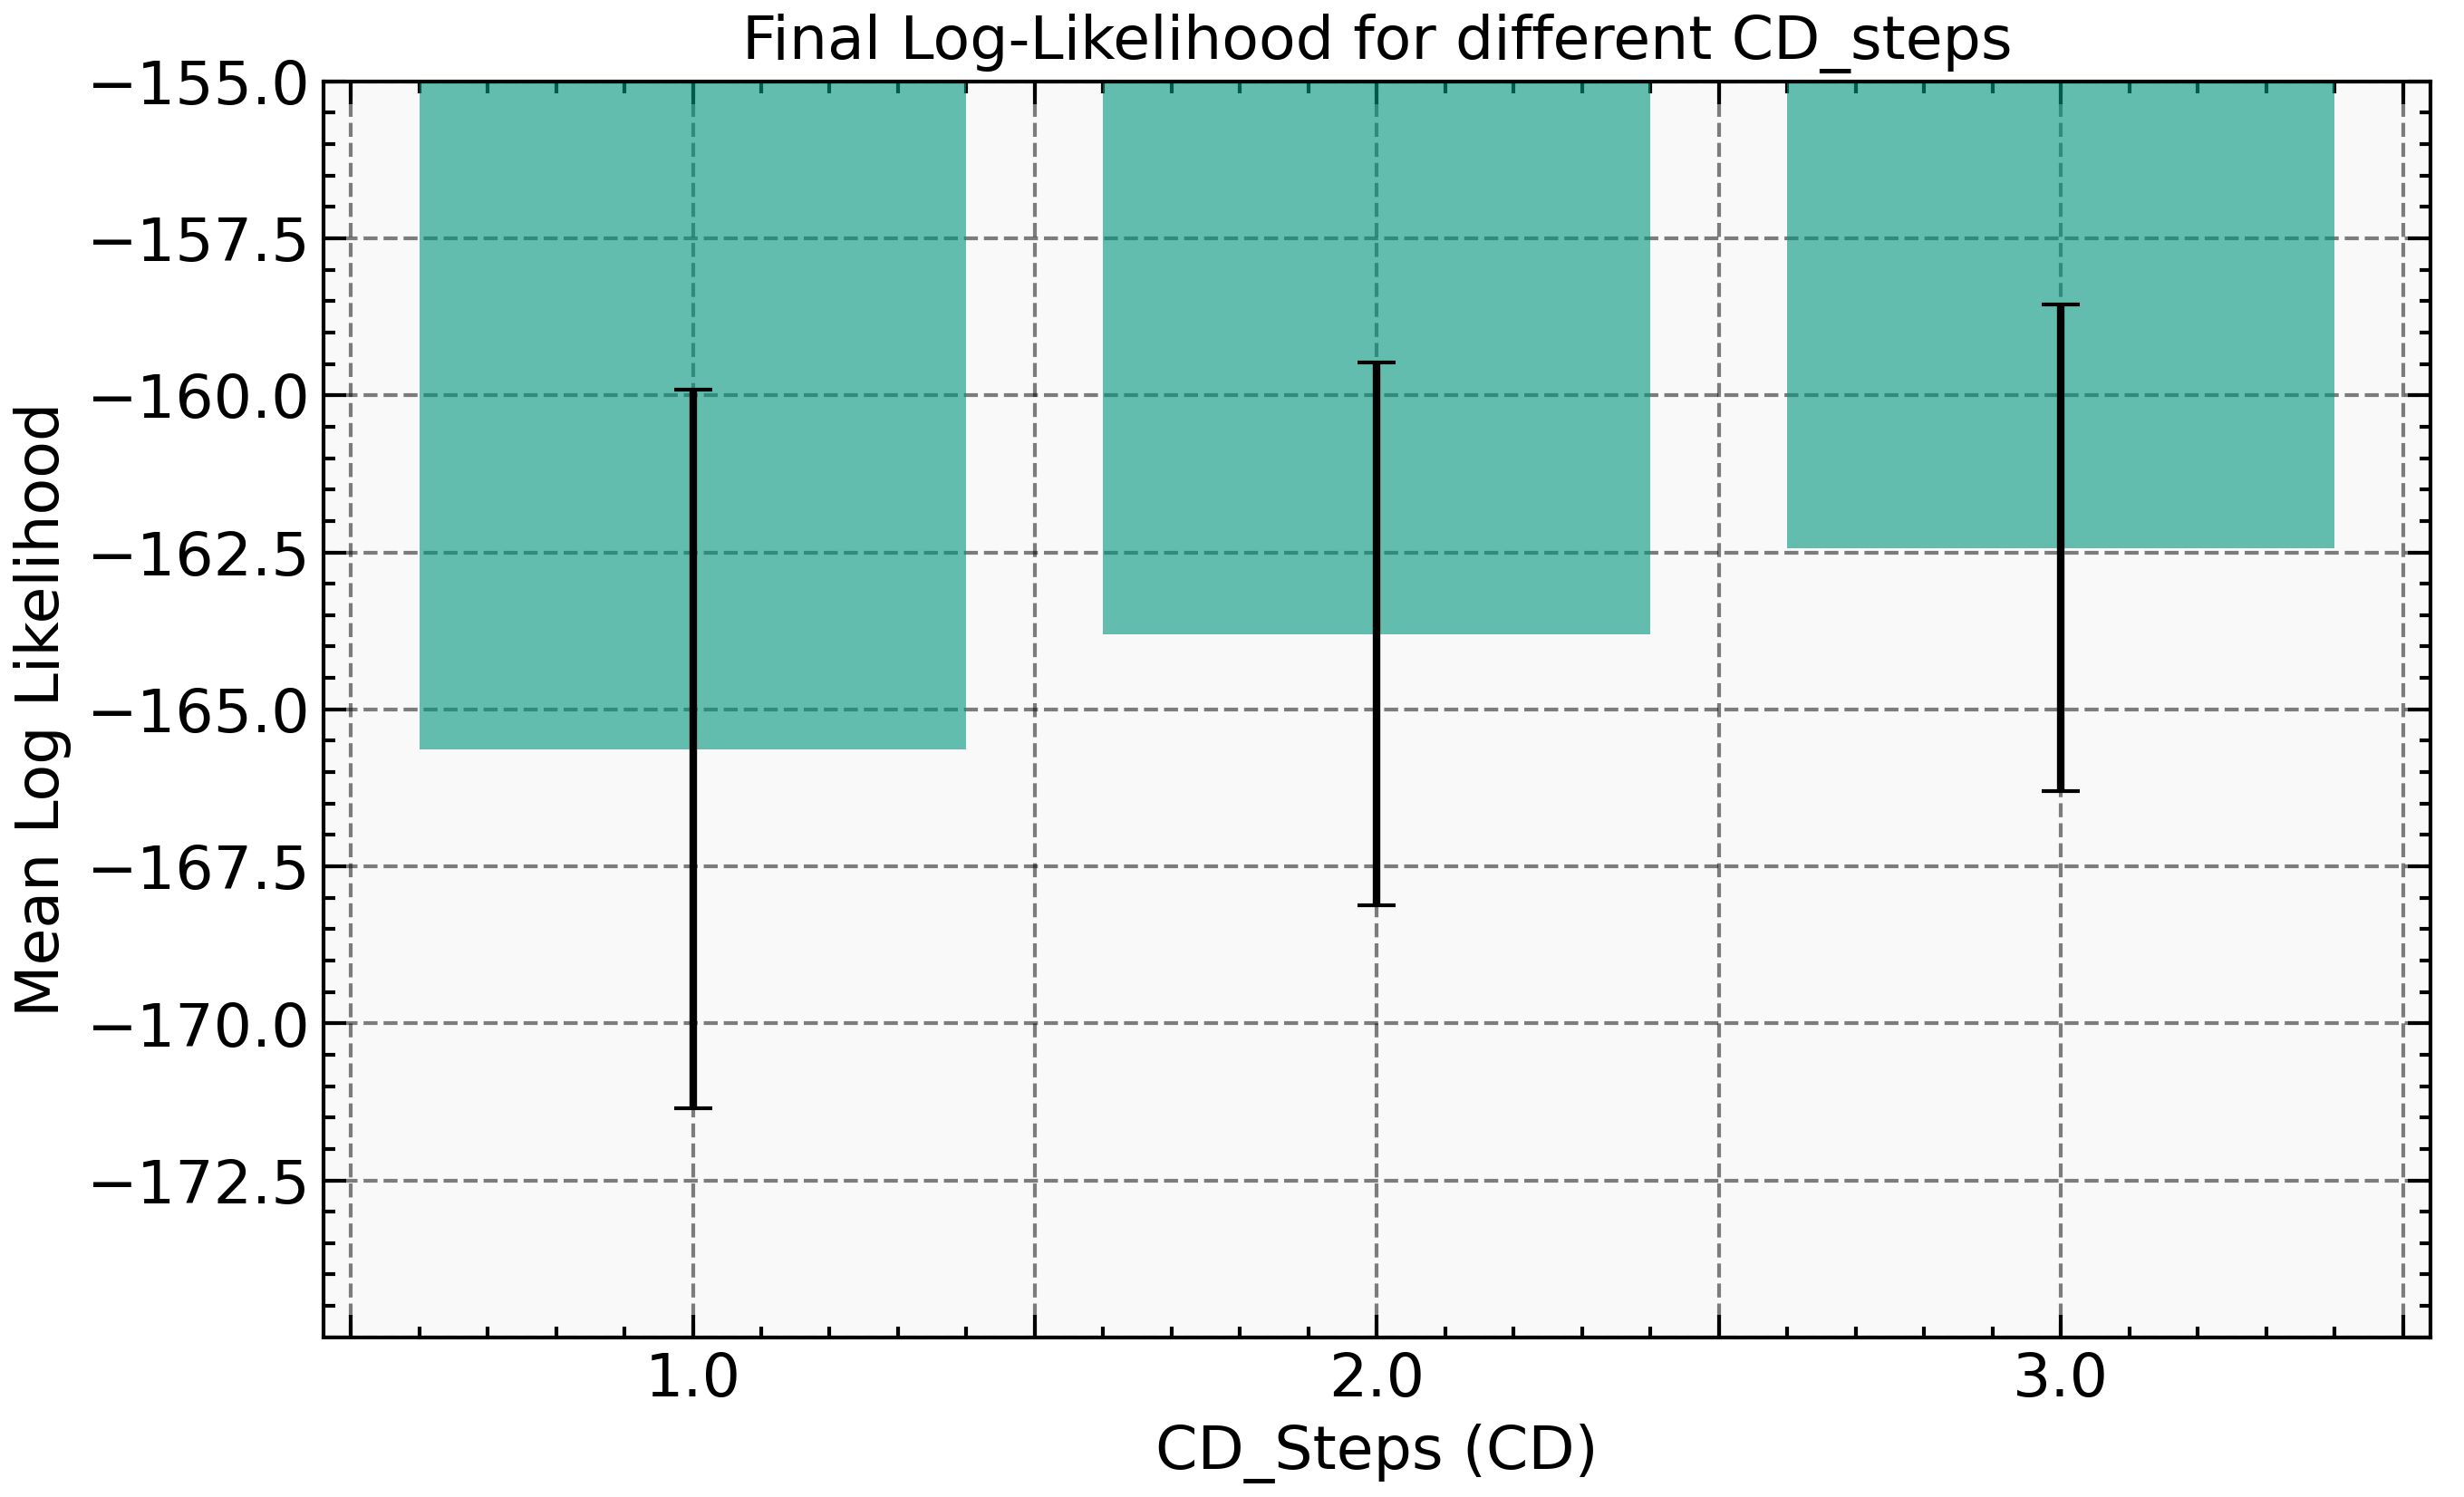
\includegraphics[width=0.465\textwidth]{final_L_of_CD.png}
	\caption{Bar chart displaying the weighted mean and standard deviation of the log-likelihood over the last epochs for different numbers of CD steps.}
	\label{fig:final_L_of_CD}
\end{figure}
%%%%%%%%%%%%%%%%%%%

where $q$ is the average of $1+e^{H_i(h)}\ \ \forall{i,h}$ that we introduce to avoid overflow. Concerning the training process of RBM, $v_i$ are set using real data. Weights $w_{i\mu}$ are initialized sampling values from a Gaussian distribution of mean $0$ and standard deviation of $2/\sqrt{L+D}$. Biases $b_\mu$ of hidden units are initialized to $0$. Thus $h_\mu$ are evaluated by Eq.~\ref{eq:p_of_h} before passed to Eq.~\ref{eq:p_of_v} in order to compute back $v_i$. In such evaluation it is convenient to set $a_i=\log[t_i/(1-t_i)]$; fixed the $i$-th visible unit, $t_i$ is defined as the number of times such unit is $1$ over the whole training array set, normalized over the size of the set. Referring to Eq.~\ref{eq:p_of_v}, the choice of shifting the sigmoid $\sigma(x)$ by the function $\log[t_i/(1-t_i)]$ of the average $t_i$ ensures that the units can activate properly, even given initial weights $w_{i\mu}$ close to $0$.

The initialization of biases $a_i$, firstly proposed by Hinton \cite{pap2}, makes hidden units able to activate and differentiate better their activation based on data, avoiding the risk of getting stuck on values near to $0$.
\\
\\
\\
\noindent\textbf{3.2. Computation}
\\
\\
We define two Python3 classes, one for the computation of the log-likelihood and the other for defining the RBM structure and managing all the input and output of the training process. Referring to Eq.~\ref{eq:loglikelihood}, in order to address the problem of overflow of $e^{H_i(h)v_i}$, we approximate the summation of powers over $h$ as a sum of the biggest ones. The purpose of this choice is to extract the biggest term out of the summation thus the applied logarithm avoids exponentiation.

Regarding the expression of the partition function shown in Eq.~\ref{eq:Z_function_bernulli}, it changes form in Spin case, since it is characterized by units taking values from $\{-1,1\}$; manipulating the second member of the equation one gets:

\begin{equation}
	Z=\sum_v\sum_h{e^{-E(v,h)}}=\sum_h{G(h)\prod_{i=1}^D{2\cosh(H_i(h))}}
	\label{eq:Z_function_spin}
\end{equation}

For Eq.~\ref{eq:Z_function_spin} the $2\cosh(H_i(h))$ term is approximated to just $e^{H_i(h)}$ by adding a common positive value to all the exponents, which shifts them away from negative domain, and compensating that out of the summation. Thus the same approximation procedure described for Eq.~\ref{eq:loglikelihood} is applied to Eq.~\ref{eq:Z_function_spin}.

%%%%%%%%%%%%%%%%%%%
\begin{figure}[!tb]
	
\includegraphics[width=0.44\textwidth]{fig1a.png}
	\caption{Description...}
	\label{fig:y}
\end{figure}
%%%%%%%%%%%%%%%%%%%

To upload the values of the weights and biases during the training phase, we adopted two different gradient descent types: SGD and RMSprop, whose update equations are found in the Appendix (Eq.~\ref{eq:sgd} and Eq.~\ref{eq:rmsprop}); we adopt the versions with the “+” sign, for gradient ascent, since we aim to maximize a monotonically increasing function. The LASSO regularization (Eq.~\ref{eq:regu}), controlled by the constant $\gamma$, is performed after applying gradient ascent during training.

We define a function to visualize the evolution of the log-likelihood of a specific model throughout the training phase and another function to compute and display the mean log-likelihood and standard deviation over the last few epochs. For our analysis, we select the set of digits $\{0,1,2\}$ from the MNIST database. We then evaluate the performance of the RBM by utilizing the visualization functions to compare different configurations of hyperparameters. In order to account for stochasticity, for each chosen set of hyperparameters we first perform ten independent training runs varying the NumPy random seed and then compute the mean log-likelihood accross runs obtaining an average trend. To derive a final log-likelihood value for each hyperparmeter configuration, we calculate a weighted average of the values of the log-likelihood over the last few training epochs. Specifically, we examine the influence of variations in the number of Contrastive Divergence steps (CD), in the number $L$ of hidden units and in parameters such as the learning rate $\eta$, $\epsilon$ and $\gamma$; here $\epsilon$ is a coefficient in the RMSprop update rule (see Eq.~\ref{eq:rmsprop}).

%%%%%%%%%%%%%%%%%%%
\begin{figure}[!tb]
	
\includegraphics[width=0.44\textwidth]{fig1a.png}
	\caption{Description...}
	\label{fig:z}
\end{figure}
%%%%%%%%%%%%%%%%%%%

Additionally, we analyze the impact of the optimizer choice for models with one-hot encoding enabled (POTTS) or disabled and either Bernoulli or Spin variables.


\section{4. Results}


Describe what you found.

Cite Figure~\ref{fig:x}(a), etc. to add information. Later also cite Figure~\ref{fig:y} and  Figure~\ref{fig:z}. Of course the number and size of figures may vary from project to project.

Cite Table~\ref{tab:1} to collect useful data in a clear way.

  zzzzzzzzzzzzzzz zzzzz zzzzzzzzzz zzzzzzz z zzzzzzzzzzz zzzz zzzzzzzzz
  zzzzzzzzzzzzzzz zzzzz zzzzzzzzzz zzzzzzz z zzzzzzzzzzz zzzz zzzzzzzzz
  zzzzzzzzzzzzzzz zzzzz zzzzzzzzzz zzzzzzz z zzzzzzzzzzz zzzz zzzzzzzzz
  zzzzzzzzzzzzzzz zzzzz zzzzzzzzzz zzzzzzz z zzzzzzzzzzz zzzz zzzzzzzzz
  zzzzzzzzzzzzzzz zzzzz zzzzzzzzzz zzzzzzz z zzzzzzzzzzz zzzz zzzzzzzzz.

  zzzzzzzzzzzzzzz zzzzz zzzzzzzzzz zzzzzzz z zzzzzzzzzzz zzzz zzzzzzzzz
  zzzzzzzzzzzzzzz zzzzz zzzzzzzzzz zzzzzzz z zzzzzzzzzzz zzzz zzzzzzzzz
  zzzzzzzzzzzzzzz zzzzz zzzzzzzzzz zzzzzzz z zzzzzzzzzzz zzzz zzzzzzzzz
  zzzzzzzzzzzzzzz zzzzz zzzzzzzzzz zzzzzzz z zzzzzzzzzzz zzzz zzzzzzzzz
  zzzzzzzzzzzzzzz zzzzz zzzzzzzzzz zzzzzzz z zzzzzzzzzzz zzzz zzzzzzzzz.
  zzzzzzzzzzzzzzz zzzzz zzzzzzzzzz zzzzzzz z zzzzzzzzzzz zzzz zzzzzzzzz
  zzzzzzzzzzzzzzz zzzzz zzzzzzzzzz zzzzzzz z zzzzzzzzzzz zzzz zzzzzzzzz
  zzzzzzzzzzzzzzz zzzzz zzzzzzzzzz zzzzzzz z zzzzzzzzzzz zzzz zzzzzzzzz
  zzzzzzzzzzzzzzz zzzzz zzzzzzzzzz zzzzzzz z zzzzzzzzzzz zzzz zzzzzzzzz
  zzzzzzzzzzzzzzz zzzzz zzzzzzzzzz zzzzzzz z zzzzzzzzzzz zzzz zzzzzzzzz.

  zzzzzzzzzzzzzzz zzzzz zzzzzzzzzz zzzzzzz z zzzzzzzzzzz zzzz zzzzzzzzz
  zzzzzzzzzzzzzzz zzzzz zzzzzzzzzz zzzzzzz z zzzzzzzzzzz zzzz zzzzzzzzz
  zzzzzzzzzzzzzzz zzzzz zzzzzzzzzz zzzzzzz z zzzzzzzzzzz zzzz zzzzzzzzz
  zzzzzzzzzzzzzzz zzzzz zzzzzzzzzz zzzzzzz z zzzzzzzzzzz zzzz zzzzzzzzz
  zzzzzzzzzzzzzzz zzzzz zzzzzzzzzz zzzzzzz z zzzzzzzzzzz zzzz zzzzzzzzz.

  

  zzzzzzzzzzzzzzz zzzzz zzzzzzzzzz zzzzzzz z zzzzzzzzzzz zzzz zzzzzzzzz
  zzzzzzzzzzzzzzz zzzzz zzzzzzzzzz zzzzzzz z zzzzzzzzzzz zzzz zzzzzzzzz
  zzzzzzzzzzzzzzz zzzzz zzzzzzzzzz zzzzzzz z zzzzzzzzzzz zzzz zzzzzzzzz
  zzzzzzzzzzzzzzz zzzzz zzzzzzzzzz zzzzzzz z zzzzzzzzzzz zzzz zzzzzzzzz
  zzzzzzzzzzzzzzz zzzzz zzzzzzzzzz zzzzzzz z zzzzzzzzzzz zzzz zzzzzzzzz.


  zzzzzzzzzzzzzzz zzzzz zzzzzzzzzz zzzzzzz z zzzzzzzzzzz zzzz zzzzzzzzz
  zzzzzzzzzzzzzzz zzzzz zzzzzzzzzz zzzzzzz z zzzzzzzzzzz zzzz zzzzzzzzz
  zzzzzzzzzzzzzzz zzzzz zzzzzzzzzz zzzzzzz z zzzzzzzzzzz zzzz zzzzzzzzz
  zzzzzzzzzzzzzzz zzzzz zzzzzzzzzz zzzzzzz z zzzzzzzzzzz zzzz zzzzzzzzz
  zzzzzzzzzzzzzzz zzzzz zzzzzzzzzz zzzzzzz z zzzzzzzzzzz zzzz zzzzzzzzz.
  zzzzzzzzzzzzzzz zzzzz zzzzzzzzzz zzzzzzz z zzzzzzzzzzz zzzz zzzzzzzzz
  zzzzzzzzzzzzzzz zzzzz zzzzzzzzzz zzzzzzz z zzzzzzzzzzz zzzz zzzzzzzzz
  zzzzzzzzzzzzzzz zzzzz zzzzzzzzzz zzzzzzz z zzzzzzzzzzz zzzz zzzzzzzzz
  zzzzzzzzzzzzzzz zzzzz zzzzzzzzzz zzzzzzz z zzzzzzzzzzz zzzz zzzzzzzzz
  zzzzzzzzzzzzzzz zzzzz zzzzzzzzzz zzzzzzz z zzzzzzzzzzz zzzz zzzzzzzzz.
  
  zzzzzzzzzzzzzzz zzzzz zzzzzzzzzz zzzzzzz z zzzzzzzzzzz zzzz zzzzzzzzz
  zzzzzzzzzzzzzzz zzzzz zzzzzzzzzz zzzzzzz z zzzzzzzzzzz zzzz zzzzzzzzz
  zzzzzzzzzzzzzzz zzzzz zzzzzzzzzz zzzzzzz z zzzzzzzzzzz zzzz zzzzzzzzz
  zzzzzzzzzzzzzzz zzzzz zzzzzzzzzz zzzzzzz z zzzzzzzzzzz zzzz zzzzzzzzz
  zzzzzzzzzzzzzzz zzzzz zzzzzzzzzz zzzzzzz z zzzzzzzzzzz zzzz zzzzzzzzz.

  


  zzzzzzzzzzzzzzz zzzzz zzzzzzzzzz zzzzzzz z zzzzzzzzzzz zzzz zzzzzzzzz
  zzzzzzzzzzzzzzz zzzzz zzzzzzzzzz zzzzzzz z zzzzzzzzzzz zzzz zzzzzzzzz
  zzzzzzzzzzzzzzz zzzzz zzzzzzzzzz zzzzzzz z zzzzzzzzzzz zzzz zzzzzzzzz
  zzzzzzzzzzzzzzz zzzzz zzzzzzzzzz zzzzzzz z zzzzzzzzzzz zzzz zzzzzzzzz
  zzzzzzzzzzzzzzz zzzzz zzzzzzzzzz zzzzzzz z zzzzzzzzzzz zzzz zzzzzzzzz.

\section{5. Conclusions}

Discuss the key aspects that we can take home from this work.

Check if your text is light, swift, and correct in exposing its passages.


\section{Appendix}

\begin{equation}
	\boldsymbol{\theta}_{t+1}=\boldsymbol{\theta}_t-\gamma\cdot{\eta_t}\cdot{\mathsf{sign}(\boldsymbol{\theta})}
	\label{eq:regu}
\end{equation}

\begin{equation}
	\boldsymbol{\theta}_{t+1}=\boldsymbol{\theta}_t\pm\eta_t\nabla_{\boldsymbol{\theta}}{E(\boldsymbol{\theta})}
	\label{eq:sgd}
\end{equation}


\begin{equation}
	\begin{cases}
		\boldsymbol{g}_t=\nabla_{\boldsymbol{\theta}}{E(\boldsymbol{\theta})} \\
		\boldsymbol{s}_t=\beta{\boldsymbol{s}_{t-1}}+(1-\beta)\boldsymbol{g}_t^2 \\
		\boldsymbol{\theta}_{t+1}=\boldsymbol{\theta}_t\pm\eta_t\frac{\boldsymbol{g}_t}{\sqrt{\boldsymbol{s}_t+\epsilon}}
	\end{cases}
	\label{eq:rmsprop}
\end{equation}


\begin{thebibliography}{99}

\bibitem{pap1}
	Pankaj Mehta,
	Marin Bukov,
	Ching-Hao Wang,
	Alexandre G.R. Day,
	Clint Richardson,
	Charles K. Fisher,
	David J. Schwab,
	\textit{A high-bias, low-variance introduction to Machine Learning for physicists},
	Physics Reports {\bf 810}, 1--124 (2019).
  
\bibitem{pap2}
	Geoffrey E. Hinton,
	\textit{A Practical Guide to Training Restricted Boltzmann Machines},
	Neural Networks: Tricks of the Trade: Second Edition, 599--619 (2012).

\end{thebibliography}

\clearpage


\end{document}